\chapter{Related Work}\label{chaprelatedwork}

% table comparing the approaches
% * laziness
% * polymorphism
% * annotations (required / supported)
% * decidability
% * errors generated

\section{Neil Mitchell's \emph{Catch}}

Neil Mitchel's \emph{Catch} (``CAse Totality CHecker'') \cite{Mitchell} is a tool specialized in finding potential pattern match failures in Haskell programs.

\subsection{Overview}

Catch works by calculates preconditions on functions. The preconditions are given in a constraint language. By varying the constraint language trade-offs between performance and precision can be made. If the calculated precondition for |main| is True, the program does not crash.

Preconditions are calculated iteratively. Precondition start out as |True|, except for |error|, whose precondition is |False|.\footnote{Note that |undefined| is defined in terms of |error|.}

\paragraph{Example} Following the example given by Mitchell, given the function:
\begin{code}
safeTail xs =  case null xs of
                  True   -> []
                  False  -> tail xs
\end{code}
the computed precondition will be:
\[ \textrm{Precondition}(|null xs|) \land (|null xs| \in \{|True|\} \lor \textrm{Precondition}(|tail xs|)), \]
stating the necessary precondition for |null xs| not to crash must be fulfilled and either |null xs| must evaluate to |True| or the necessary precondition for |tail xs| not to crash must be fulfilled.

As |null xs| cannot crash we find its precondition to be simply True and we can deduce the precondition for |tail xs| to be $|xs|\in\{(:)\}$. Substituting these into our precondition we find
\[ \textrm{True} \land (|null xs| \in \{|True|\} \lor |xs|\in\{(:)\}), \]
which simplifies to
\[ |null xs| \in \{|True|\} \lor |xs|\in\{(:)\}. \]
The subexpression  $|null xs| \in \{|True|\}$ forms a postcondition on |null xs|. From this postcondition Catch computes the required precondition that satisfies it, which in this particular case should turn out to be $|xs|\in\{[]\}$. Substituting, we find
\[ |xs|\in\{[]\} \lor |xs|\in\{(:)\}, \]
which, using our knowledge of the list data type, turns out the be a tautology, i.e. the (trivial) precondition for |safeTail| is True.

\subsection{Constraint Systems}
The example in the previous section used a simple constraint language, specifying to which set of head constructors an expression should evaluate. Mitchell developed two more expressive constraint systems: regular expression constraints and multipattern constraints.

\paragraph{Regular expression constraints} Constraints are formed by a regular expression over an alphabet of a number of ad-hoc \emph{selectors} (e.g. |hd| and |tl| for lists.) A precondition for |map head xs| using regular expression constraints reads $|xs| \in (|tl|^{*} \cdot |hd| \leadsto \{(:)\})$. It should be interpreted as ``after applying zero or more |tl|s to |xs| and then applying a |hd| we should find a |(:)| constructor.''

According to Mitchell regular expression constraints tend to scale badly as the program increase in size, although he could not identify more specific condition under which this problem manifests.\footnote{Personal communication}

\paragraph{Multipattern constraints} Multipatterns are of the form $\alpha \star \rho$, where $\alpha$ gives the set of constructors that are valid at the head of the value, while $\rho$ gives the set of constructors that can appear at the recursive positions (if any) of the constructor at the head of the value. The elements of these sets can again be multipatterns. To specify that |xs| in |map head xs| should be a list of non-empty lists, we use the multipattern:
\begin{align*}
\{[]&, (:) (\{(:)\ |Any| \} \star \{ [], (:)\ |Any|\})\} \\
&\star \\
\{[]&, (:) (\{(:)\ |Any| \} \star \{ [], (:)\ |Any|\})\}
\end{align*}
|Any| is a wildcard that matches any constructor.

\subsection{Discussion}
% should have been mentioned earlier?
The analysis of Catch works on a first-order language. The input program needs to be defunctionalized before it can be analyzed. The defunctionalization algorithm employed by Catch is not complete.

Calculated preconditions are unnecessarily restrictive in the presence of laziness (Mitchell, p. 142).


\section{Static Contract Checking}
\subsection{Overview}
Dana Xu's work on static contract checking for Haskell \cite{Xu09staticcontract} (including the ESC/Haskell system \cite{Xu:2006:ESC:1159842.1159849}) allows checking of arbitrary programmer supplied pre- and postconditions on functions and is able to detect pattern match failures in the process.

Programmers define pre- and postconditions in the form of a contract (a refinement type). An appropriate contract for the |head| function defined above might be:
\begin{verbatim}
{-# CONTRACT head :: {s | not (null s)) -> {x | True} #-}
\end{verbatim}
This contract states that if head is given a list |s| for which the predicate |not (null s)| holds, i.e. it is a non-empty list, the function will not crash\footnote{The system only guarantees partial correctness, so the term might still diverge.}, indicated by the trivial postcondition |True| on the return value.

\begin{figure}
\centering
\begin{tabular}{lclr}
t &$::=$& $\{ x || p \}$     & Predicate          \\
  & $||$ & $x : t_1 \to t_2$ & Dependent function  \\
  & $||$ & $(t_1, t_2)$      & Constructor         \\
  & $||$ & $Any$             & Polymorphic ``Any''
\end{tabular}
\caption{Syntax of Xu's contracts}
\label{xu-contract-syntax}
\end{figure}

Contracts can be constructed from predicates, a dependent function space constructor, arbitrary constructors and a polymorphic |Any| contract that is always satisfied, including by functions which crash (Fig. \ref{xu-contract-syntax}). Any |Bool|-valued Haskell expression can be used as a predicate.

Dependent functions are helpful when declaring a contract, e.g. for the |reverse| function:
\begin{verbatim}
{-# CONTRACT reverse
      :: {xs | True} -> {rs | length xs == length rs} #-}
\end{verbatim}
The predicate on the return value depends on the input. Constructors and the |Any| contract are useful when declaring a contract for |fst|:
\begin{verbatim}
{-# CONTRACT fst :: (Ok, Any) -> Ok #-}
\end{verbatim}
Here |Ok| is used as a shorthand for |{x || True}|. As |fst| discards the value on the right in the tuple we should not care if it is an expression that crashes, so we can not use |Ok|.

\subsection{Contract Checking}
Haskell's syntax is extended with two \emph{exception values}---|BAD| and |UNR|---which are only used internally by the checker. |BAD| signifies an expression which crashes and |UNR| an expression which is either unreachable or diverges.

In the program that is going to be verified all crashing expressions (including |error| and |undefined|), as well as missing patterns in case-expressions are replaced by |BAD| exceptions.

The verification of the contracts is based on a translation of the contracts into Findler--Felleisen wrappers \cite{Findler:2002:CHF:581478.581484}, which will cause a function to crash (using |BAD|) if it disobeys its contract or diverge if it called in a way that is not permitted. While technically interesting it is not directly relevant to the detection of pattern match failures so we shall not discuss it in more depth.

The actual verification process continues by \emph{symbolic evaluation}, basically applying various simplifications to the resulting program including $\beta$-reductions. Any code deemed to be unreachable is pruned from the program.

The presence of recursive functions in the contracts might cause the symbolic evaluation to diverge if care is not taken to limit the number of evaluation steps. By setting an upper bound on the number of simplification steps we lose accuracy, but gain decidability of the verification process.

Arithmetical expressions in case-expressions (e.g. |case x * x >= 0 of { True -> ...; False -> BAD }|) cannot be handled directly by the symbolic evaluator. These are collected in a table and send to an external constraint or SMT solver. If the solver determines these expressions are inconsistent the code is unreachable and can be pruned.

After the symbolic evaluation has terminated the checker will tell the programmer if the program is ``definitely satisfies the contract'' (if no |BAD| exceptions remain anywhere in the program), ``definitely does not satisfy the contract'' or ``don't know.''

\subsection{Discussion}
Unlike our envisioned system, Xu's static contract checking requires programmer supplied contracts on nearly all functions (contracts on trivial functions can be omitted and are handled by inlining their definition when called.) Compared to Mitchell's Catch it can handle higher-order functions natively and has a more (too?) expressive contract language.

\section{Dependent ML}
DML($\mathcal{L}$) is an extension of the ML programming language which enriches ML's type system with a limited form of dependent types over a (decidable) constraint domain (or index language) $\mathcal{L}$ \cite{DML-JFP07}.

Xi's initial example---recast in a more Haskell-like syntax---declares a |List| data type dependent on an integer corresponding to the length of the list and a function to concatenate two such lists:
\begin{verbatim}
type Nat = {a :: Int | a >= 0}

data List<Int> a = Nil<0>
                 | {n :: Nat} Cons<n+1> a (List<n> a)

(++) :: {m :: Nat} {n :: Nat} List<m> a -> List<n> a -> List<m+n> a
(++) Nil         ys = ys
(++) (Cons x xs) ys = Cons x (append xs ys)
\end{verbatim}


For many functions producing a list, the exact length might not be derived by such a trivial calculation (|m+n|) on the lengths of the input lists. A prominent example is the |filter| function:
\begin{verbatim}
filter :: (a -> Bool) -> {m :: Nat} List<m> a
                      -> [n :: Nat | n <= m] List<n> a
filter p Nil         = Nil
filter p (Cons x xs) | p x       = Cons x (filter p xs)
                     | otherwise =         filter p xs
\end{verbatim}
here we only know that the resulting list is equal or shorter in length than the input list (|n <= m|). This is expressed as the dependent sum |[n :: Nat || n <= m]|. In a full-fledged dependently-typed language we would also return a proof object stating the predicate |p| holds for all the elements in the output list, but this is beyond the expressive power of DML.

What we gain is a relief from the need to provide proofs for trivial arithmetical (in)equalities. Imagine a |zip| function which requires the two list to be zipped together to be of equal length. When calling |zip (xs ++ ys) (ys ++ xs)| this precondition seems to be intuitively satisfied. From the point-of-view of the compiler the first list has length $m+n$ and the second lists $n+m$, however. In most dependently-typed languages we will now have to invoke a lemma or tactic proving the commutativity of addition. DML can simply send the constraint $m + n = n + m$ to an ILP solver and conclude the constraint is satisfiable.

\subsection{Discussion}
Compared to Xu's static contract checking, Xi's DML constrains the constraint system to a decidable theory. The constraints and indices---such as |m+n| and |n <= m|---may superficially look like ordinary Haskell expression, but in fact belong to a much smaller index language. While type checking is decidable, type inference is not and as a result DML still requires type annotations.

To be applicable to a pattern match analysis we must try to infer a type like:
\begin{verbatim}
head :: {n :: Int || n >= 1} [a]<n> -> a
\end{verbatim}
for the |head| function. We also have to implicitly extend the list data type with an index representing its length.

This seems significantly more challenging than inferring the Catch-like type
\begin{alltt}
head :: \{xs :: [a] || xs \(\in\) (:) \} -> a
\end{alltt}
The correspondence between the type and the pattern matching happening in the definition of |head| is much more direct.

\section{Refinement Types}\label{secrt}

\begin{figure}[t]
\centering
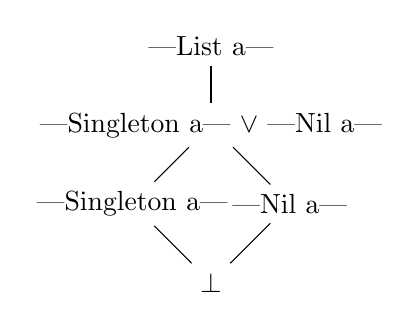
\begin{tikzpicture}
    \tikzstyle{all nodes}=[inner sep=4pt]
    \draw node(top)at(1,3){|List a|}
          node(sorn)at(1,2){{|Singleton a|} $\lor$ {|Nil a|}}
          node(s)at(0,1){|Singleton a|} node(n)at(2,1){|Nil a|}
          node(bot)at(1,0){$\bot$};
    \draw[-](top)--(sorn);
    \draw[-](sorn)--(s);
    \draw[-](sorn)--(n);
    \draw[-](s)--(bot);
    \draw[-](n)--(bot);
\end{tikzpicture}
\caption{A lattice of {|List|} and its {|rectype|}s.}
\label{listlattice}
\end{figure}


Refinement types are a form of subtyping that allow us to state more accurately what values a variable of a particular type can contain. For example, a refinement type {\tt \{ a :: Int || a < 0 \}} states that |a| is a variable of type |Int| that can only contain negative numbers.

Freeman and Pfenning \cite{Freeman:1991:RTM:113445.113468,Freeman94refinementtypes} give a formal development of refinement types for the ML programming language that can support recursive types.

Their key contribution is allowing the programmer to define |rectype|s. Besides defining a recursive type for lists:

\begin{verbatim}
data List a = Nil || Cons a (List a)
\end{verbatim}

the programmer can also define a |rectype| describing singleton lists:

\begin{verbatim}
rectype Singleton a = Cons a Nil
\end{verbatim}

Together with an automatically derived |rectype| for the non-recurisive constructor |Nil| (and a union type contructor) the compiler can construct---using known algorithms on regular tree grammars \cite{DBLP:books/others/tree1984}---a finite lattice of refinement types for |List a| given in Figure \ref{listlattice}.

\subsection{Union and Intersection Types}\label{secit}

Refinement types are constructed from regular types, including function types, as well as union and intersection types.

A union type such as {\tt Int $\lor$ Bool}, {\tt List a $\lor$ Singleton a} or {\tt Int -> Int $\lor$ Bool -> Bool} state that a value can be either of the type on the left or of the type on the right, but we do not know which. In the case of {\tt List a $\lor$ Singleton a} we are able to simplify this type to {\tt List a}, as {\tt Singleton a} is a subtype of {\tt List a}.

An intersection type such as {\tt Int $\land$ Bool}, {\tt List a $\land$ Singleton a} or {\tt Int -> Int $\land$ Bool -> Bool} state the a value has both the type on the left and the type on the right. Compared to union types these are more interesting. The type {\tt List a $\land$ Singleton a} can still be simplified, but now to {\tt Singleton a}. A value cannot be of both type {\tt Int} and {\tt Bool}, so we can simply the type of such a value to the bottom or empty type. There do exist functions that are of both type {\tt Int -> Int} and {\tt Bool -> Bool}, for example {\tt id}. In fact, intersection types can in the limit be viewed as a form of parametric polymorphism.

\subsection{Constructors and Pattern Matching}

To infer refinement types more accurate types need to be given to constructors. This is done by using a restricted\footnote{We only take intersections of subtypes of the same data type.} form of intersection types. For example, the {\tt Cons} constructor is given the type:

\begin{verbatim}
Cons  ::  a  -> Nil        a  -> Singleton  a
      &&  a  -> Singleton  a  -> List       a
      &&  a  -> List       a  -> List       a
\end{verbatim}

This type can be derived automatically from the |rectype| declarations. Types of functions can also be inferred automatically, although there may be a loss of precision when higher-order functions or polymorphism are involved.

Type inference for intersection types is undecidable in general \cite{Pierce91programmingwith,Reynolds96designof}. Because the lattice of types is finite the algorithm is effectively able to do an exhaustive search over all possible types, however. Higher-order functions can cause the size of the type to blow up exponentially, each pairing of their range and domain needs to be included in the intersection type.

A case-statement 

\begin{verbatim}
case G of
  Nil        -> E1
  Cons a as  -> E2
\end{verbatim}

can be seen as a call to a higher-order function

\begin{verbatim}
case_List G E1 (\a as -> E2)
\end{verbatim}

where |case_List| has the refinement type

\begin{verbatim}
case_List :: forall a. forallR (r1 :: a). forallR (r2 :: a).
       Nil a       -> r1 -> (List a -> r2) -> r1
    /\ Singleton a -> r1 -> (List a -> r2) -> r2
    /\ List a      -> r1 -> (List a -> r2) -> (r1 \/ r2)
\end{verbatim}

\section{Compiling Pattern Matching}
Case-statements in toy languages often have a very simple \emph{decision tree} semantics. Case-statements in Haskell have a more complex \emph{backtracking automaton} semantics. There is a body of work on compiling the latter into the former. Maranget \cite{DBLP:journals/jfp/Maranget07} gives an algorithm for determining whether a case-statement is exhaustive and whether all patterns are useful. As the analysis does not consider any dataflow information it is much too imprecise for our purpose. It does turn out that the analysis closely follows, but can at places be simplified with respect to, the manner in which pattern matching is compiled. This indicates we might also be able to follow such an approach when analyzing case-statements in our pattern-match analysis.
